% Created 2023-04-12 Wed 10:29
% Intended LaTeX compiler: pdflatex
\documentclass[14pt]{extarticle}
\usepackage[utf8]{inputenc}
\usepackage[T2A]{fontenc}
\usepackage{graphicx}
\usepackage{longtable}
\usepackage{wrapfig}
\usepackage{rotating}
\usepackage[normalem]{ulem}
\usepackage{amsmath}
\usepackage{amssymb}
\usepackage{capt-of}
\usepackage{hyperref}
\usepackage[russian]{babel}
\usepackage{tempora}
\usepackage{geometry}
\geometry{a4paper, left=30mm, top=20mm, bottom=20mm, right=15mm }
\usepackage{graphicx}
\usepackage{array}
\usepackage{tabularx}
\usepackage{listings}
\usepackage{float}
\usepackage{setspace}
\usepackage{tabularx}
\usepackage{longtable}
\usepackage{titlesec}
\titleformat*{\section}{\large\bfseries}
\titleformat*{\subsection}{\normalsize\bfseries}
\titleformat*{\subsubsection}{\normalsize\bfseries}
\addto\captionsrussian{\renewcommand{\contentsname}{\centering \normalsize СОДЕРЖАНИЕ}}
\addtocontents{toc}{\protect\thispagestyle{empty}}
\usepackage{titletoc}
\titlecontents{section}[0pt]{}{\contentsmargin{0pt} \thecontentslabel\enspace}{\contentsmargin{0pt}}{\titlerule*[0.5pc]{.}\contentspage}[]
\dottedcontents{subsection}[3.1em]{}{1.5em}{0.5pc}
\usepackage{caption}
\DeclareCaptionLabelSeparator{custom}{ -- }
\captionsetup[figure]{name=Рисунок, labelsep=custom, font={onehalfspacing}, justification=centering}
\usepackage{ragged2e}
\justifying
\setlength\parindent{1.25cm}
\sloppy
\usepackage{indentfirst}
\usepackage{multirow}
\usepackage{lscape}
\author{Панков Вася}
\date{\today}
\title{02.02. Инструментальные средства разработки}
\hypersetup{
 pdfauthor={Панков Вася},
 pdftitle={02.02. Инструментальные средства разработки},
 pdfkeywords={},
 pdfsubject={У. С. Опалева},
 pdfcreator={Emacs 30.0.50 (Org mode 9.6.2)}, 
 pdflang={Russian}}

% Setup for code blocks [1/2]

\usepackage{fvextra}

\fvset{%
  commandchars=\\\{\},
  highlightcolor=white!95!black!80!blue,
  breaklines=true,
  breaksymbol=\color{white!60!black}\tiny\ensuremath{\hookrightarrow}}

% Make line numbers smaller and grey.
\renewcommand\theFancyVerbLine{\footnotesize\color{black!40!white}\arabic{FancyVerbLine}}

\usepackage{xcolor}

% In case engrave-faces-latex-gen-preamble has not been run.
\providecolor{EfD}{HTML}{f7f7f7}
\providecolor{EFD}{HTML}{28292e}

% Define a Code environment to prettily wrap the fontified code.
\usepackage[breakable,xparse]{tcolorbox}
\DeclareTColorBox[]{Code}{o}%
{colback=EfD!98!EFD, colframe=EfD!95!EFD,
  fontupper=\footnotesize\setlength{\fboxsep}{0pt},
  colupper=EFD,
  IfNoValueTF={#1}%
  {boxsep=2pt, arc=2.5pt, outer arc=2.5pt,
    boxrule=0.5pt, left=2pt}%
  {boxsep=2.5pt, arc=0pt, outer arc=0pt,
    boxrule=0pt, leftrule=1.5pt, left=0.5pt},
  right=2pt, top=1pt, bottom=0.5pt,
  breakable}

% Support listings with captions
\usepackage{float}
\floatstyle{plain}
\newfloat{listing}{htbp}{lst}
\newcommand{\listingsname}{Listing}
\floatname{listing}{\listingsname}
\newcommand{\listoflistingsname}{List of Listings}
\providecommand{\listoflistings}{\listof{listing}{\listoflistingsname}}


% Setup for code blocks [2/2]: syntax highlighting colors

\newcommand\efstrut{\vrule height 2.1ex depth 0.8ex width 0pt}
\definecolor{EFD}{HTML}{212121}
\definecolor{EfD}{HTML}{FAFAFA}
\newcommand{\EFD}[1]{\textcolor{EFD}{#1}} % default
\definecolor{EFh}{HTML}{607d8b}
\newcommand{\EFh}[1]{\textcolor{EFh}{#1}} % shadow
\definecolor{EFsc}{HTML}{4eee94}
\newcommand{\EFsc}[1]{\textcolor{EFsc}{#1}} % success
\definecolor{EFw}{HTML}{FF5722}
\newcommand{\EFw}[1]{\textcolor{EFw}{#1}} % warning
\definecolor{EFe}{HTML}{B71C1C}
\newcommand{\EFe}[1]{\textcolor{EFe}{#1}} % error
\definecolor{EFc}{HTML}{607d8b}
\newcommand{\EFc}[1]{\textcolor{EFc}{#1}} % font-lock-comment-face
\definecolor{EFcd}{HTML}{607d8b}
\newcommand{\EFcd}[1]{\textcolor{EFcd}{#1}} % font-lock-comment-delimiter-face
\definecolor{EFs}{HTML}{689f38}
\newcommand{\EFs}[1]{\textcolor{EFs}{#1}} % font-lock-string-face
\definecolor{EFd}{HTML}{673ab7}
\newcommand{\EFd}[1]{\textcolor{EFd}{#1}} % font-lock-doc-face
\definecolor{EFm}{HTML}{558b2f}
\newcommand{\EFm}[1]{\textcolor{EFm}{#1}} % font-lock-doc-markup-face
\definecolor{EFk}{HTML}{00796b}
\newcommand{\EFk}[1]{\textcolor{EFk}{#1}} % font-lock-keyword-face
\definecolor{EFb}{HTML}{B71C1C}
\newcommand{\EFb}[1]{\textcolor{EFb}{#1}} % font-lock-builtin-face
\definecolor{EFf}{HTML}{0097A7}
\newcommand{\EFf}[1]{\textcolor{EFf}{#1}} % font-lock-function-name-face
\definecolor{EFv}{HTML}{EF6C00}
\newcommand{\EFv}[1]{\textcolor{EFv}{#1}} % font-lock-variable-name-face
\definecolor{EFt}{HTML}{0097A7}
\newcommand{\EFt}[1]{\textcolor{EFt}{#1}} % font-lock-type-face
\definecolor{EFo}{HTML}{558b2f}
\newcommand{\EFo}[1]{\textcolor{EFo}{#1}} % font-lock-constant-face
\definecolor{EFwr}{HTML}{B71C1C}
\newcommand{\EFwr}[1]{\textcolor{EFwr}{\textbf{#1}}} % font-lock-warning-face
\definecolor{EFnc}{HTML}{2196f3}
\newcommand{\EFnc}[1]{\textcolor{EFnc}{#1}} % font-lock-negation-char-face
\definecolor{EFpp}{HTML}{FFA000}
\newcommand{\EFpp}[1]{\textcolor{EFpp}{#1}} % font-lock-preprocessor-face
\definecolor{EFrc}{HTML}{4527A0}
\newcommand{\EFrc}[1]{\textcolor{EFrc}{#1}} % font-lock-regexp-grouping-construct
\definecolor{EFrb}{HTML}{FFA000}
\newcommand{\EFrb}[1]{\textcolor{EFrb}{#1}} % font-lock-regexp-grouping-backslash
\definecolor{Efob}{HTML}{EFEBE9}
\newcommand{\EFob}[1]{\colorbox{Efob}{\efstrut{}#1}} % org-block
\newcommand{\EFhn}[1]{#1} % highlight-numbers-number
\newcommand{\EFhq}[1]{#1} % highlight-quoted-quote
\newcommand{\EFhs}[1]{#1} % highlight-quoted-symbol
\newcommand{\EFrda}[1]{#1} % rainbow-delimiters-depth-1-face
\newcommand{\EFrdb}[1]{#1} % rainbow-delimiters-depth-2-face
\newcommand{\EFrdc}[1]{#1} % rainbow-delimiters-depth-3-face
\newcommand{\EFrdd}[1]{#1} % rainbow-delimiters-depth-4-face
\newcommand{\EFrde}[1]{#1} % rainbow-delimiters-depth-5-face
\newcommand{\EFrdf}[1]{#1} % rainbow-delimiters-depth-6-face
\newcommand{\EFrdg}[1]{#1} % rainbow-delimiters-depth-7-face
\newcommand{\EFrdh}[1]{#1} % rainbow-delimiters-depth-8-face
\newcommand{\EFrdi}[1]{#1} % rainbow-delimiters-depth-9-face
\begin{document}

\begin{titlepage}

\centering{ГУАП}

\vspace{32pt}

\centering{ФАКУЛЬТЕТ СРЕДНЕГО ПРОФЕССИОНАЛЬНОГО ОБРАЗОВАНИЯ}

\vspace{60pt}

\raggedright{ОТЧЕТ \\
ЗАЩИЩЕН С ОЦЕНКОЙ}
\vspace{14pt}

\raggedright{ПРЕПОДАВАТЕЛЬ}

\vspace{12pt}

\begin{tabularx}{\textwidth}{ >{\centering\arraybackslash}X >{\centering\arraybackslash}X >{\centering\arraybackslash}X }
	 преподаватель & & У. С. Опалева \\ 
	 \hrulefill & \hrulefill & \hrulefill \\ 
\footnotesize{должность, уч. степень, звание} & \footnotesize{подпись, дата} & \footnotesize{инициалы, фамилия} \\ 
\end{tabularx} 
 
\vspace{48pt} 

\centering{ОТЧЕТЫ О ЛАБОРАТОРНЫХ РАБОТАХ} 

\vspace{76pt} 

\centering{По дисциплине: 02.02. Инструментальные средства разработки} 

\vspace*{\fill} 

\raggedright{РАБОТУ ВЫПОЛНИЛ} 

\vspace{10pt} 

\begin{tabularx}{\textwidth}{>{\raggedright\arraybackslash}X  >{\centering\arraybackslash}X >{\centering\arraybackslash}X >{\centering\arraybackslash}X }
	 СТУДЕНТ ГР. № & 021к & & Панков Вася \\ 
	 & \hrulefill & \hrulefill & \hrulefill \\ 
	 &  & \footnotesize{подпись, дата} & \footnotesize{инициалы, фамилия} \\ 
\end{tabularx} 
 
\vspace*{\fill} 

\centering{Санкт-Петербург \the\year} 

\end{titlepage}

\tableofcontents \clearpage

\section{Лабораторная работа №5-6}
\label{sec:org14b88b7}


Тема: Разработка и интеграция модулей проекта. Отладка отдельных модулей ПП. Организация обработки исключений.

\begin{enumerate}
\item Открыть в VS проект, созданный по шаблону Bottle в п.1-6 предыдущей ЛР.
Вызвать окно свойств отладки либо так, как предложено в разделе теоретических сведений, либо как показано на скриншоте ниже:

\begin{figure}[H]
\centering
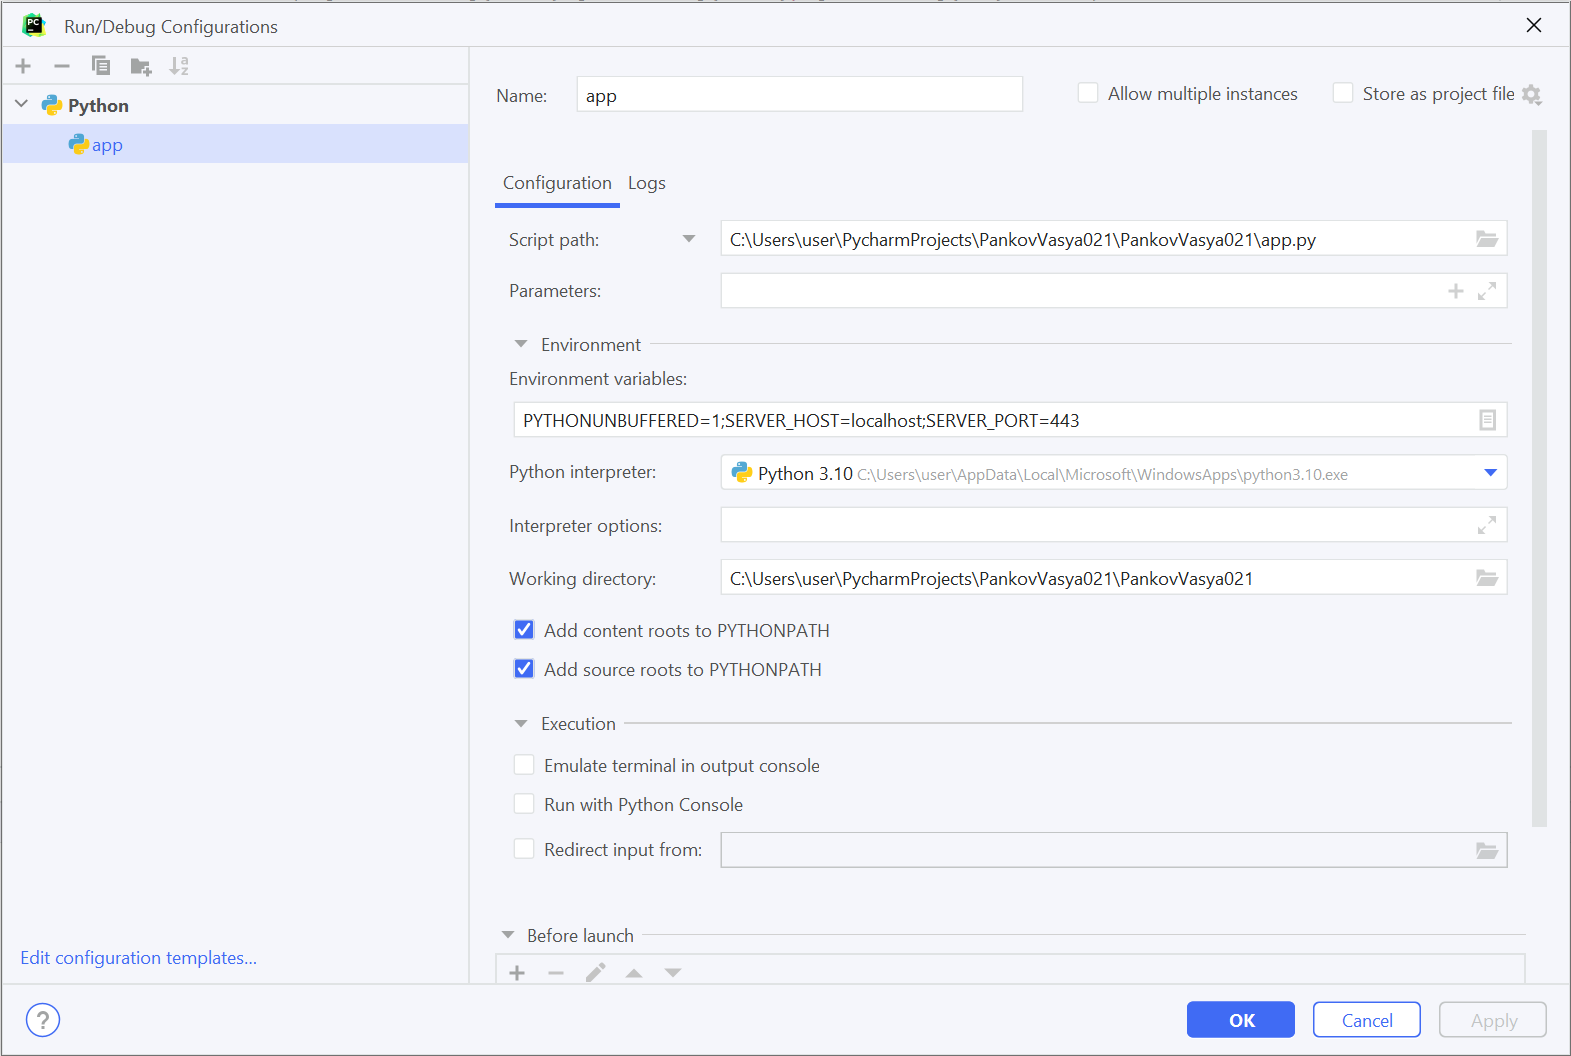
\includegraphics[width=.9\linewidth]{images/2023-04-12_09-41-37_screenshot.png}
\caption{Окно свойств отладки}
\end{figure}

\item В открывшемся окне свойств отладки с помощью всплывающих подсказок изучить
описания параметров и те их значения, которые заданы по умолчанию. Результаты внести в отчёт.

\begin{itemize}
\item Sript path - путь для запускаемого файла

\item Parameters - параметры запуска

\item Enviroment variables - переменнные среды

\begin{itemize}
\item PYTHONUNBUFFERED

\item SERVER\textsubscript{HOST} - переменнная, среды, которая берётся в нашей программе,
для определения ip адреса, где будет запущена программа

\item SERVER\textsubscript{PORT} - переменнная, среды, которая берётся в нашей программе,
для определения номера порта, который будет прослушивать наша программа
\end{itemize}

\item Python interpreter - выбор интерпритатора python

\item Interpreter options - параметры запуска для интерпретатора

\item Working directory - рабочая папка

\item Content root – Это коллекция файлов, из которых можно импортировать модули

\item Source root – Директория, в которой хранятся ресурсы.

\item Галочки, означают, добавление Специального параметра – PYTHONPATH, при вызове

\item Emulate terminal - эмуляция терминала

\item Run with Python Console – вывод внешней питоновской консоли

\item Redirect input – позволяет указать файл, из которого будет браться программный ввод

\item Before launch – позволяет перед запуском конфигурации запустить браузер, внешний инструмент или даже другую конфигурацию
\end{itemize}
\item Установить фиксированный номер порта, например, 443:
\begin{figure}[H]
\centering
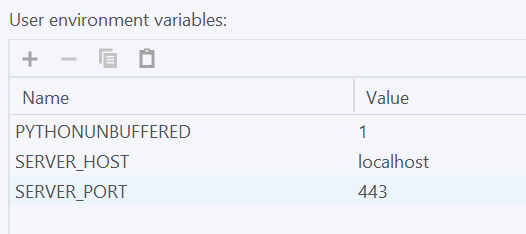
\includegraphics[width=.9\linewidth]{images/2023-04-12_09-55-16_screenshot.png}
\caption{Установил переменные среды}
\end{figure}

\begin{figure}[H]
\centering
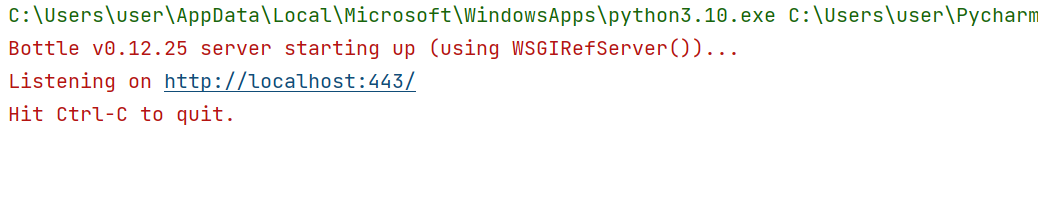
\includegraphics[width=.9\linewidth]{images/2023-04-12_09-56-02_screenshot.png}
\caption{После изменения порта}
\end{figure}

\begin{figure}[H]
\centering
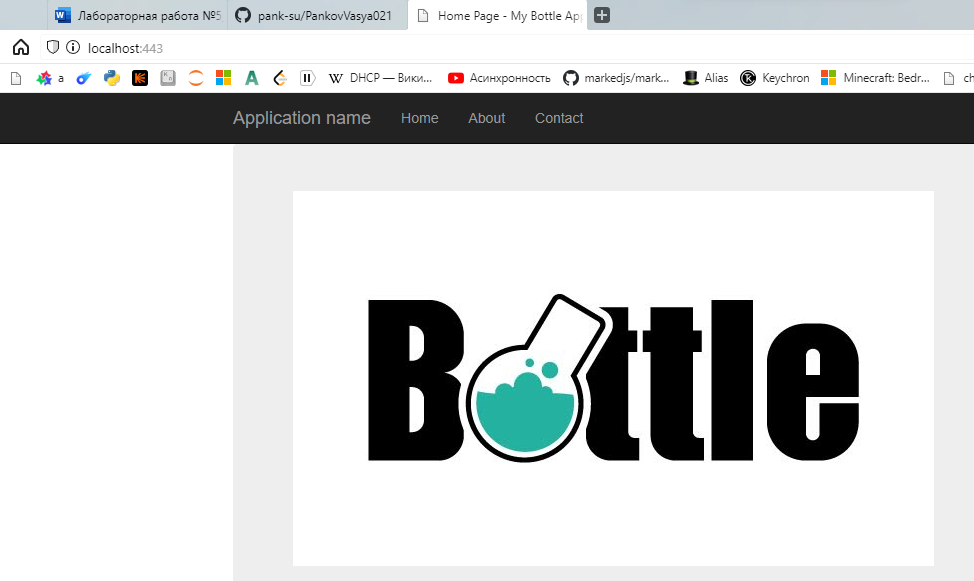
\includegraphics[width=.9\linewidth]{images/2023-04-12_09-58-11_screenshot.png}
\caption{Изменённый порт в браузере}
\end{figure}

\begin{figure}[H]
\centering
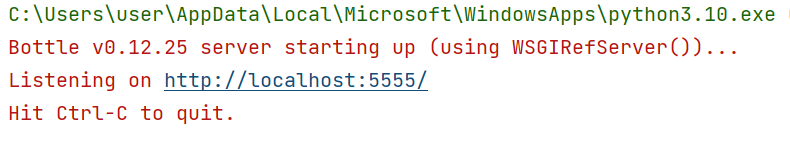
\includegraphics[width=.9\linewidth]{images/2023-04-12_09-57-31_screenshot.png}
\caption{Порт по умолчанию}
\end{figure}
\item Добавить на главную страницу сайта простейшую форму обратной связи, состоящую из текстовой области, текстового поля и кнопки.

Выяснить, что означают атрибуты HTML-тэгов, сделать размер textarea неизменяемым.
\begin{itemize}
\item action – Какую функцию апи выполнить

\item method – Какой http-метод используется(get, post, put)

\item rows, cols - Кол-во рядов и колонок текста

\item name – указывает имя для элемента html

\item plaseholder – текст-подсказка

\item type – у тэга input позволяет выбрать конкретный элемент формы(checkbox, date, file и тд)

\item value – значение которое пишется внутри тэга
\end{itemize}

\begin{figure}[H]
\centering

\includegraphics[width=.9\linewidth]{images/2023-04-12_10-01-19_screenshot.png}
\caption{Textarea неизменяемый по содержанию и по размеру}
\end{figure}

\begin{figure}[H]
\centering
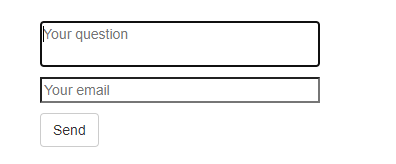
\includegraphics[width=.9\linewidth]{images/2023-04-12_10-02-56_screenshot.png}
\caption{Итоговая форма}
\end{figure}

Выполнить коммит изменений. Показать в отчёте историю коммитов.

\begin{figure}[H]
\centering
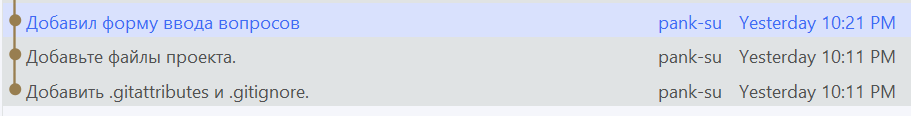
\includegraphics[width=.9\linewidth]{images/2023-04-12_10-05-03_screenshot.png}
\caption{История коммитов}
\end{figure}
\item Теперь необходимо добавить в папку проекта файл-обработчик для формы.

\begin{figure}[H]
\centering
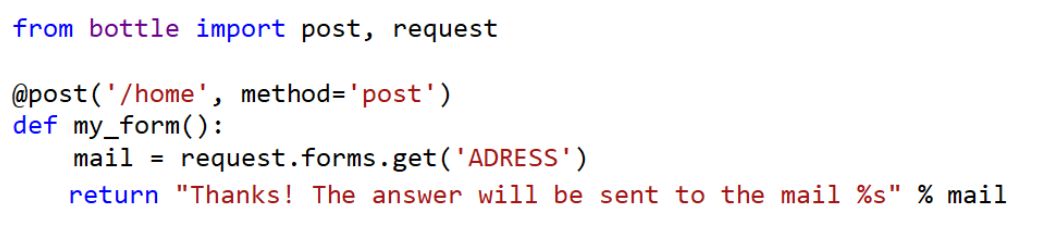
\includegraphics[width=.9\linewidth]{images/2023-04-12_10-07-45_screenshot.png}
\caption{Форма}
\end{figure}

\item Тестирование формы

\begin{figure}[H]
\centering
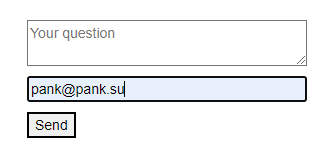
\includegraphics[width=.9\linewidth]{images/2023-04-12_10-08-25_screenshot.png}
\caption{Вставка email}
\end{figure}

\begin{figure}[H]
\centering

\includegraphics[width=.9\linewidth]{images/2023-04-12_10-09-51_screenshot.png}
\caption{Результат обработки формы}
\end{figure}

\item Дописать в файл обработчик:

\begin{enumerate}
\item Паттерн для адреса электронной почты (проверку на соответствие формату).

\begin{figure}[H]
\centering
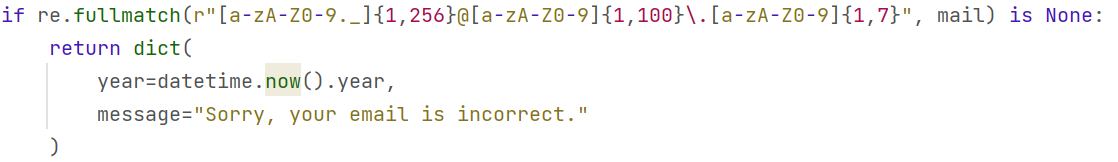
\includegraphics[width=.9\linewidth]{images/2023-04-12_10-11-04_screenshot.png}
\caption{Проверка почты на корректность}
\end{figure}

\item Обращение по имени в результирующем сообщении, например, «Thanks, Nik! …»,
предварительно дописав необходимый элемент вёрстки «USERNAME» в шаблоне страницы.
При тестировании вводить своё имя, набранное на латинице.

Было добавлен получение поля username и добавление его в строку вывода:

\begin{center}
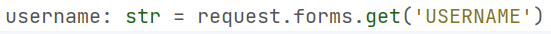
\includegraphics[width=.9\linewidth]{images/2023-04-12_10-17-27_screenshot.png}
\end{center}
\begin{center}
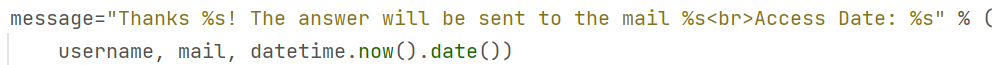
\includegraphics[width=.9\linewidth]{images/2023-04-12_10-17-16_screenshot.png}
\end{center}

\item Дату обращения пользователя в сокращённом формате согласно текущей системной дате в конце результирующего сообщения, например, «… Access Date: 2023-02-22».

Получаю сегодняшнее время с помощью datetime и получаю из этого времени дату:

\begin{center}
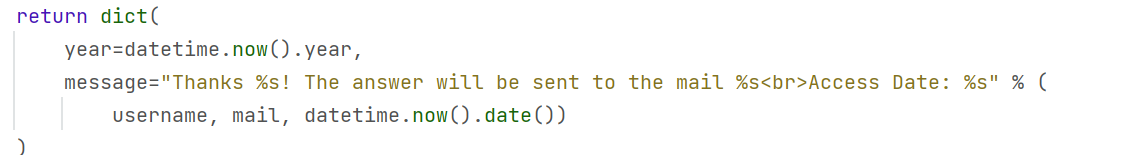
\includegraphics[width=.9\linewidth]{images/2023-04-12_10-18-37_screenshot.png}
\end{center}

\item Проверку заполненности полей формы (если хотя бы одно поле не заполнено выводить соответствующее сообщение).

\begin{figure}[H]
\centering
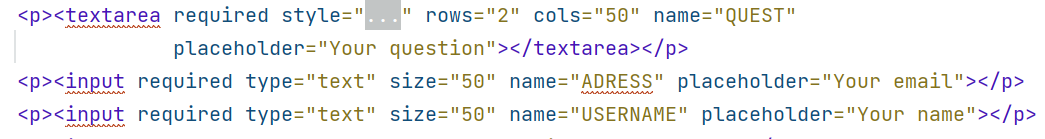
\includegraphics[width=.9\linewidth]{images/2023-04-12_10-14-53_screenshot.png}
\caption{Добавлен required на каждое поле ввода}
\end{figure}
\end{enumerate}
\end{enumerate}



Итоговый код формы:

\begin{Code}
\begin{Verbatim}
\color{EFD}\EFk{import} re

\EFk{from} bottle \EFk{import} post, request, view
\EFk{from} datetime \EFk{import} datetime


\EFt{@post}(\EFs{'/home'}, method=\EFs{'post'})
\EFt{@view}(\EFs{"index"})
\EFk{def} \EFf{my\_form}():
    \EFv{mail}: \EFb{str} = request.forms.get(\EFs{'ADRESS'})
    \EFv{username}: \EFb{str} = request.forms.get(\EFs{'USERNAME'})
    \EFk{if} re.fullmatch(r\EFs{"[a-zA-Z0-9.\_]\{1,256\}@[a-zA-Z0-9]\{1,100\}\char92{}.[a-zA-Z0-9]\{1,7\}"}, mail) \EFk{is} \EFo{None}:
        \EFk{return} \EFb{dict}(
            year=datetime.now().year,
            message=\EFs{"Sorry, your email is incorrect."}
        )
    \EFk{return} \EFb{dict}(
        year=datetime.now().year,
        message=\EFs{"Thanks \%s! The answer will be sent to the mail \%s<br>Access Date: \%s"} \% (
            username, mail, datetime.now().date())
    )
\end{Verbatim}
\end{Code}

​8. Выполнить тестирование исключительных ситуаций (поля не заполнены, Email не соответствует формату) и отладку кода. Закоммитеть изменения. Все результаты внести в отчёт.

Тестирование:
\begin{figure}[H]
\centering
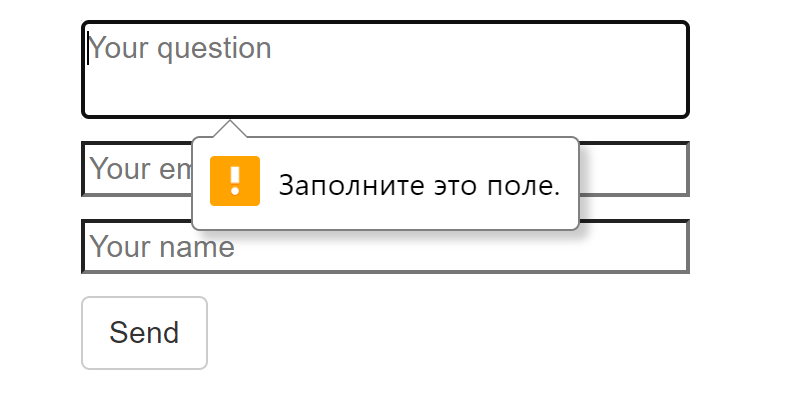
\includegraphics[width=.9\linewidth]{images/2023-04-12_10-22-27_screenshot.png}
\caption{Поля не заполнены}
\end{figure}

\begin{figure}[H]
\centering
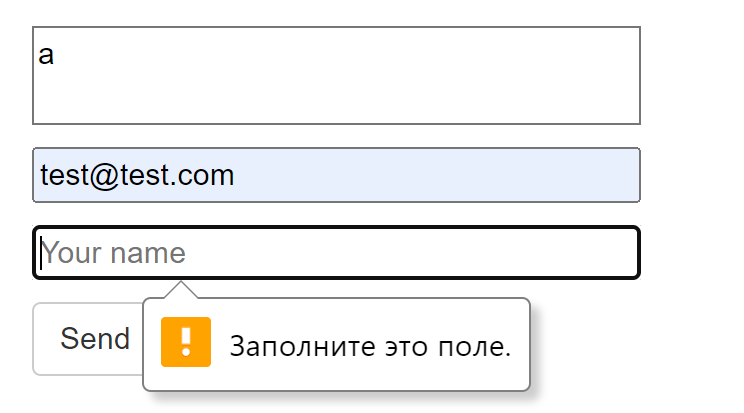
\includegraphics[width=.9\linewidth]{images/2023-04-12_10-23-09_screenshot.png}
\caption{Одно поле не заполнено}
\end{figure}

\begin{figure}[H]
\centering
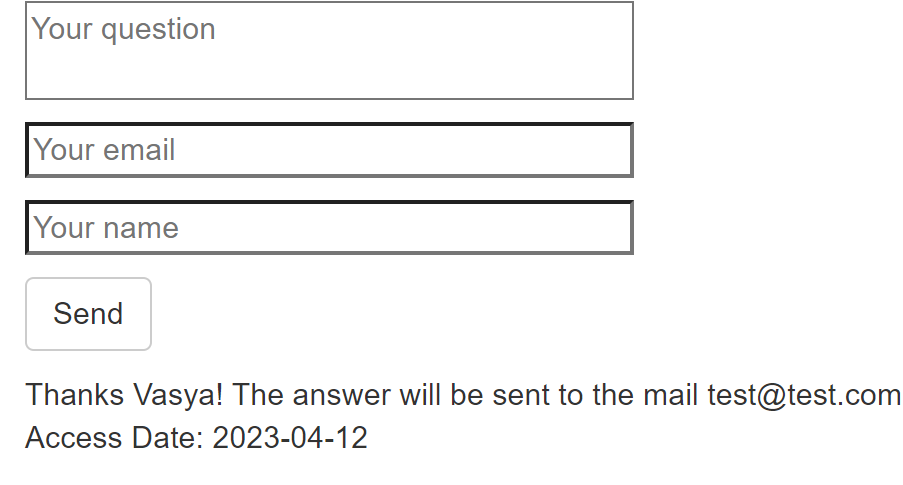
\includegraphics[width=.9\linewidth]{images/2023-04-12_10-23-44_screenshot.png}
\caption{Корректное срабатывание}
\end{figure}

\begin{figure}[H]
\centering
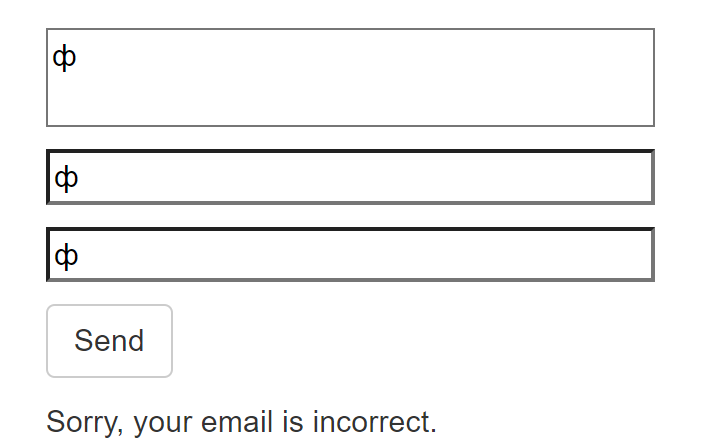
\includegraphics[width=.9\linewidth]{images/2023-04-12_10-24-31_screenshot.png}
\caption{Некорректная почта}
\end{figure}



История коммитов:
\begin{center}
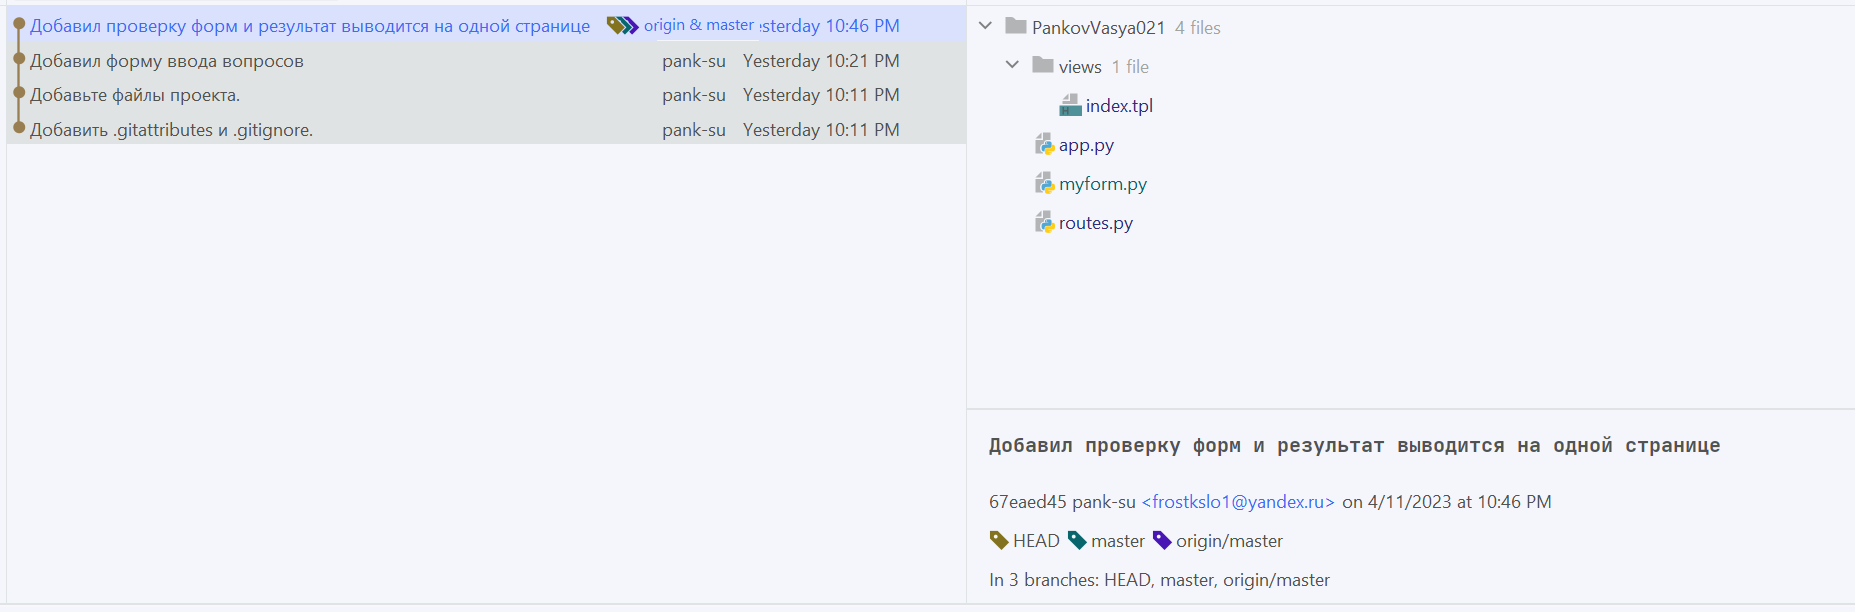
\includegraphics[width=.9\linewidth]{images/2023-04-12_10-19-58_screenshot.png}
\end{center}


Контрольные вопросы:
\begin{enumerate}
\item Какие параметры включает группа «Отладка» вкладки «Веб-средство запуска»?

Пути поиска, Аргументы сценария, Аргументы интерпретатора, Путь к
Интерпретатору, URL-адрес для запуска, Номер порта, Команда, Аргументы, Среда
\item Какого рода исключительные ситуации вам известны? Привести 3-4 примера.
Деление на ноль(ZeroDivisionError), Неправильное значение(ValueError), Несуществующее имя(NameError)
\item Как будет выглядеть регулярное выражение Python для проверки формата номера мобильного телефона +7 (ххх) ххх-хх-хх?
Например, как: \texttt{r“\textbackslash{}+7 \textbackslash{}([0-9]\{3\}\textbackslash{}) [0-9]\{3\}-[0-9]\{2\}-[0-9]\{2\}”}
\end{enumerate}
\end{document}